

\section{Селективное лазерное спекание}
\subsection{Технология}
Процесс печати изделия изображен схематически на рис. \ref{fig:printer}.\\
Описание. 


\begin{figure}[h]
    \centering
    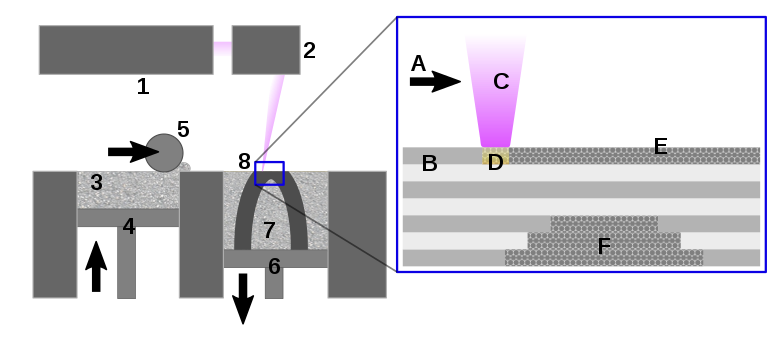
\includegraphics[width=\linewidth]{fig/sls.png}
    \caption{Caption}
    \label{fig:printer}
\end{figure}
анизотропия, слои\\
чтоб успевало спекаться (не спалвляться!!!)\\
Спекание отличается о сравнения

\subsection{Модель}

The high intensity of
the laser beam makes it possible to rapidly heat a small
region, inducing a disequilibrium of the temperature
distribution and large temperature gradients.\cite{sls-sim2016}
\\
The simulation
results showed a big difference in the temperature distributions
of composite powders, especially in terms of melting depth.\\
The experimental investigation became more
efficient due to the process predictions. The accuracy of the model
was validated by the microstructures of PA, PA/CF and PA/NaCl.
With the increasing research into various composites, this numerical
method can be further used to adopt appropriate processing
parameters for the production of functional parts and then engender
significant time and material savings.
\section{Характеристиики полимеров для СЛС}

The properties of the final product obtained by the SLS technology largely depend on the properties of the original powder (morphology, size, size distribution, bulk density, thermal properties, viscosity and surface tension) and on the parameters of laser sintering (laser power, scanning speed, laser spot diameter). Particle morphology affects the spatial arrangement of powder particles (stacking degree) relative to each other. Spherical (with a smooth surface) particles have a high packing density. They provide flowability of the powder composition in systems of applying the material with minimal resistance. In addition, spherical particles are well bonded in the process of laser sintering. It was shown that during the transition from powder particles with predominantly spherical morphology to particles of irregular shape of the same material, the elastic modulus decreases by almost 40 \%.3 The spherical particles with good flowability and a high packing densities represent ideal characteristics of the starting powder for use in SLS.4 At the same time, the use of irregularly shaped particles with a large variation in their size leads to the creation of products with higher mechanical characteristics, compared to the use of mainly spherical particles with a narrow size distribution.5

\subsection{Тепловые и механические параметры}
первая глава из
\cite{termopols}


\subsection{"Тонкая" Структура}
Что ее характеризует


\subsection{Полиэфиримиды ряда R-BAPB }
		
	\begin{figure}[h]
	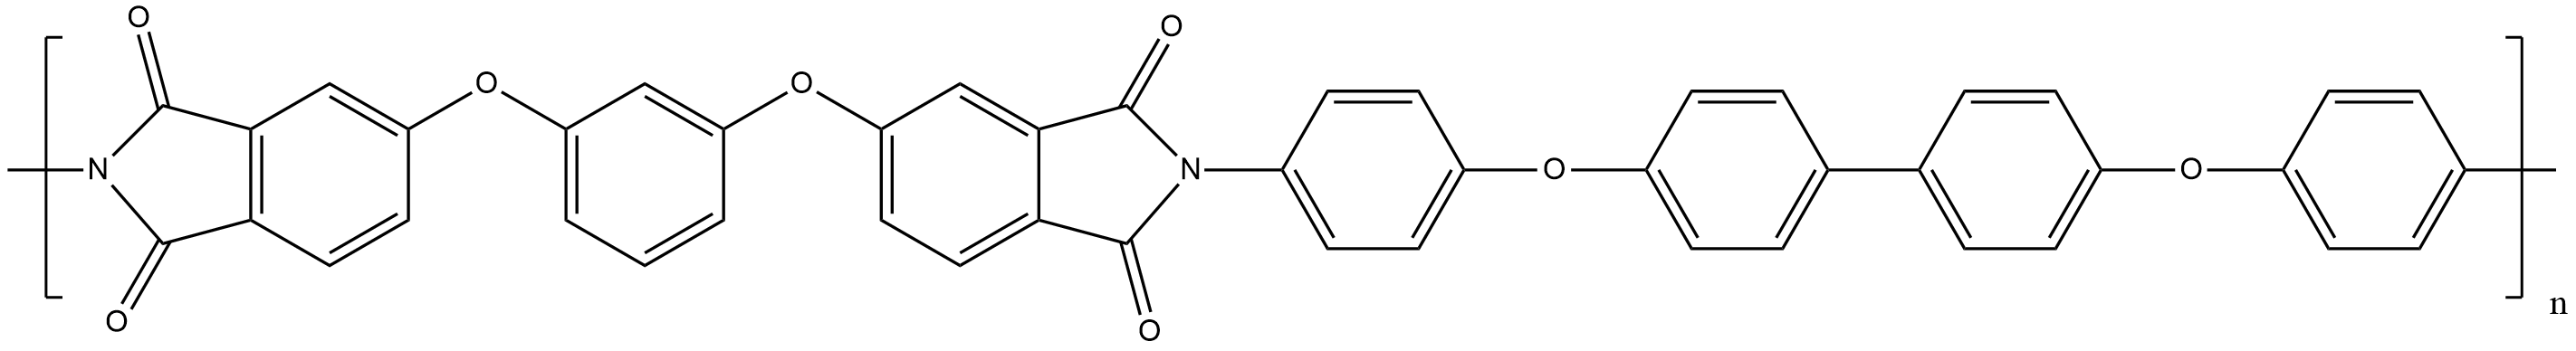
\includegraphics[width=\textwidth]{fig/formula.png}
	\end{figure}
	структура

Что следует из первичной структуры, термостойкость, особенности, пригодность для СЛС, перспективность

Данные по композитным добавкам

характеристики - все что измерили в ИВС

Что еще нужно выясеить

\subsection{Проблемы}



\section{Кристаллическая структура полимеров}

The polymer crystal structure is less perfect than crystals formed from
low-molecular-weight compounds. Polymeric materials are usually in the metastable
state, that is, they are partly crystalline and partly amorphous. Most of the polymers
are semicrystalline in structure where the crystal structure is often formed during
cooling from the melt, which controls the mechanical and physical properties of
semicrystalline polymers. Due to the high viscosity of polymer melt, polymers
crystallize very slowly at below the melting temperature (Tm), even at high supercooling.
\\
The crystal structure
and degree of crystallinity depend on the molecular structure of polymer, growth
conditions, foreign particles present in the lattice, crystallization temperature, cooling
rate, etc.\\
This can be estimated from
X-ray diffraction, density measurements, thermal analysis, etc.\\



\subsection{Кристаллиты}

The polymer crystal
morphology may be divided into lamellar and fibrillary crystals [1]. In the lamellar
crystallization process, the growth direction is perpendicular to the chain direction
and folding of chains occurs. In the fibrillary crystallization process, the growth
direction is in the chain direction and highly extended chain conformations occur in
the crystals lattice. These materials have high mechanical properties. Crystallization
changes the physical and mechanical properties of polymer systems remarkably. It is
important to note that crystallization not only occurs in linear polymer chains such
as polyethylene (PE) and poly(ethylene oxide) (PEO) but also occurs for more
complicated polymer architectures.\\
Studying the crystallization
behavior, though complicated, is necessary mainly in relation to the physical and
mechanical properties of polymers. If crystallization would be absent in polymer
systems, then the whole mechanical performance of polymers depends on the glass
transition temperature (Tg). If glass transition is the only determining factor for the
properties of the polymers, then polymers such as polypropylene (PP) and PE
would have been rubbers at ambient temperature. However, in these polymers,
due to crystallization, the stiffness is retained at acceptable and controllable values
up to the melting temperature (Tm).\\
Multiphase polymer systems commonly consist of polymer blends, composites,
nanocomposites, interpenetrating polymer networks, block copolymers, and polymer
gels. Crystallization in multicomponent polymer-based systems represents the main
physical characteristic that allows for control of the material properties.\\
The presence of nanoparticles
can also limit themotion ofmolecular chains, resulting in suppression of the crystalline
perfection and crystallinity of polymer crystals.\\
Crystallization is a first-order transition and a thermal process in polymers. The
polymer chains are aligned and folded together to form an ordered chain region,
which is called lamellae. The lamellae are composed of spherical aggregates called
spherulites. The crystallization process changes the density, symmetry, and phase
transition and thus controls the properties of the end products. Crystallization
commonly proceeds by nucleation of a fiberlike structure followed by lamellar
structure formation. The spherulites grow away from a nucleation site.\\
Nowadays polymer composites are commonly used in aerospace, sport goods, automobiles,
industrial equipment, etc. Polymer composites are polymer-based matrix
with some form of materials embedded in the matrix, as reinforcements.\\
Polymer composites are classified on the basis of the size of filler particles into
microcomposites and nanocomposites.\\
(Это в планы на будущее)
Many experimental techniques can be used to study the crystallization
kinetics of nanocomposites. The most common techniques used to study the
crystallization kinetics in the nanocomposites are DSC, optical microscopy, and
WAXD.\\
The crystallization
kinetics of polymer composites and nanocomposites gained great interest due to the
fact that fillers act as an effective nucleating agent in the polymer matrix. With the
advancement of nanotechnology, the focus is now shifting toward understanding
the crystallization properties of materials in nanodimensions and thereby tune the
properties for diversified tailored application.\\

Это все из \cite{cryst1}

	\begin{wrapfigure}{r}{0.5\textwidth} 
\vspace{-20pt}


  \begin{center}
    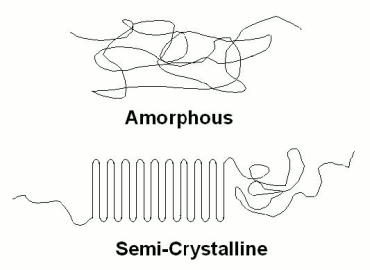
\includegraphics[width=0.4\textwidth]{fig/crystal-1.png}
    \caption{Как цепочки складываются в ламели}
    \label{fig:crystal-1}
  \end{center}
  \vspace{-20pt}
  \vspace{1pt}
\end{wrapfigure}



\begin{figure}[h]
    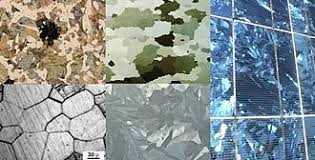
\includegraphics[width=\textwidth]{fig/crystallites.jpg}
    \caption{Типы кристаллитов}
    \label{fig:crystallites}
\end{figure}



\subsection{Частичная кристалличность}
Properties of the semicrystalline polymers can be understood, for the most part,
using a simple two-phase model that assumes that the two phases, the crystalline and
the amorphous, can be easily distinguished. If an intensive property $\phi$ (e.g., specific
volume, specific heat) of the crystalline and amorphous phases, $\phi$ c and $\phi$a, respectively, can be measured, and if we assume that contributions of the two phases
are additive, then
\[ 
\phi = \phi_c x + \phi_a(1-x)
\]
where x is the fraction of the crystalline phase, which ideally is the mass fraction
(x\_m) but depends somewhat on the technique (это из \cite{cryst3})
	
	\begin{wrapfigure}{r}{0.5\textwidth} 
\vspace{-20pt}
  \begin{center}
    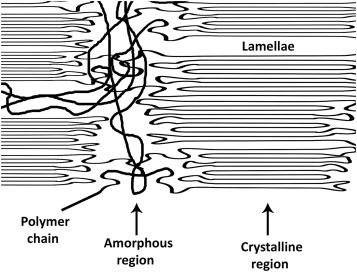
\includegraphics[width=0.4\textwidth]{fig/crystal-2.jpg}
    \caption{К определению кристалличности полимеров}
    \label{fig:crystal-2}
  \end{center}
  \vspace{-20pt}
  \vspace{1pt}
\end{wrapfigure}	

The two-phase model implied in Eq. (3.1) is only an approximation because
there can be a continuum of structures from large, defect-free single crystals to
the truly amorphous domains with liquid-like order. Because of the restrictions
imposed by long polymer chains, defects are invariably present in the crystal lattice,
and the polymer crystallites are small and disordered.\\
Conversely, the amorphous
domains possess some degree of positional and orientational correlations, and there
is experimental evidence for both rigid or ordered and soft or fluid amorphous phases\\
it may not always be possible to distinguish between the signatures
of the crystalline and amorphous phases. Nevertheless, a two-phase model with
an approximate crystalline phase and an amorphous phase, and sometimes an additional
ordered phase, mostly due to oriented amorphous domains, is often used.\\



\subsection{Влияние на макроскопические параметры}

\section{Исследование кристаллической структуры}

Тырим описание методов и формулы из \cite{cryst3}
Because the crystalline regions in these
polymers are formed from long chains, their crystallization behavior is complex
and is remarkably sensitive to small changes in the polymer composition, additives,
temperature, and mechanical forces.\\
Not all polymers
crystallize, and those that do crystallize are rarely fully crystalline: only a fraction
of the crystallizable chains are incorporated into crystalline domains and the rest
segregate into amorphous domains. The degree of crystallinity and the characteristics
of the crystalline domains are the most important morphological characteristics
that determine the physical properties such as mechanical strength, density,
processability, permeability and degradability of a semicrystalline polymer.\\
The
degree of crystallinity of a typical polymer ranges from 10\% to 80\%. This is in
contrast to those of metals that, with the exception of metallic glasses, are almost
always entirely crystalline, and ceramics that are either totally crystalline or amorphous.\\
various
commonly used techniques for measuring the crystalline content, and for understanding
some of their characteristics.\\
Polymer crystallinity can be analyzed by making use of the differences in many of
the characteristics of the crystalline and amorphous regions\\
\subsection{Плотность}
The most basic is the
small differences in the density of the crystalline and amorphous regions that makes it
possible to use density measurement for the evaluation of the polymer crystallinity.
При аддитивности по объему:
\[
\%_{x_m} =\frac{\nu - \nu_a}{\nu_c - \nu_a}\cdot100 = \frac{\rho_c}{\rho}\cdot\frac{\rho - \rho_a}{\rho_c-\rho_a}
\]
При аддитивности по массе:
\[
\%_{x_{\nu}} =\frac{\rho - \rho_a}{\rho_c-\rho_a}
\]
Точность измерения < 0.1 кг/м3\\
The density of the crystalline phase
can be calculated from the crystallographic unit cell parameters. The density of
the amorphous phase can be obtained by extrapolating to room temperature the specific
volume of the melt measured at various temperatures by dilatometric methods
[16,17]. The crystalline and the amorphous densities can also be determined experimentally
by extrapolating the densities of a series of samples with known crystallinities
as measured by XRD.\\
Короче нужен будет рса

\subsection{Термический анализ}


Equally fundamental is the thermal characteristics of the crystalline and the amorphous
regions. Because crystalline domains melt upon heating, and amorphous domains do
not, heat of fusion can be a used as a measure of the degree of crystallinity. \\
The amount of energy absorbed
depends on the degree of crystallinity. This energy can be determined using\\
differential scanning calorimetry (DSC). DSC measures the amount of heat absorbed
or released by the sample relative to a reference (an empty pan) as it is taken through
various thermal transitions at a constant heating or cooling rate, and under
isothermal conditions as a function of time.\\
The mass percent crystallinity (xm) of a specimen can be calculated from the
measured heat of fusion (DHm) and the knowledge of the value for 100\% crystalline
material $\Delta H^0_m$
from the relation
\[
\%x_m = \frac{\Delta H_m - \Delta H_c }{\Delta H^0_m}\cdot100
\]
The term DHc is the heat of cold crystallization. A typical DSC scan consists of a heat cool reheat cycle, all three being done at a rate of 10 C/min. Because materials
change during heating as well as upon cooling, the crystallinity should be determined
from the scan obtained during the first heat.\\
The implementation of Eq. (3.5)
into practice to evaluate the crystallinity is not straightforward!!!\\
issues. First, a proper baseline has to be drawn for precise determination of the crystallinity. \\
Second, crystallization of the sample during heating, cold crystallization,
is a serious problem in evaluating the crystallinities of samples with low
levels of crystalline order.\\

\subsection{Спектроскопия}
At the
structural level, the conformation of the chains is different in the crystalline and the
amorphous regions. Thus spectroscopic methods such as infrared (IR) and Raman
spectroscopy can be used to follow crystallization if the absorption bands of the chains’
crystalline and amorphous conformations can be easily identified.
\subsection{ЯМР}
Because the mobilities
of the chains in the amorphous and the crystalline regions are different, solid-state
nuclear magnetic resonance (NMR) can be used to characterize polymer crystallinity.


\subsection{Дифракция}
Finally, polymer chains are packed into crystal lattices, and these lattices, even if they
are disordered, give rise to crystalline diffraction peaks in wide-angle X-ray scattering
(WAXS) patterns. Thus the intensity of the crystalline peaks in X-ray diffraction
(XRD) can be used as a direct measure of the polymer crystallinity. In addition,
when a polymer crystallizes, it often forms large-scale structures such as lamellae
and fibrils. These larger structures can be observed using small-angle X-ray scattering
(SAXS) and electron microscopy\\
The two commonly used X-ray scattering techniques to examine the crystalline
features of semicrystalline polymers are: WAXS, also called wide-angle X-ray
diffraction (WAXD), and SAXS. WAXS is sensitive to atomic and molecular structures
and thus provides a direct measure of the crystallinity. SAXS is sensitive to
mesoscale structures and reports on the effect of changes in the crystallinity on
the morphology of the polymer.\\

\subsection{Микроскопия}
The even larger structures such as spherulites
formed by the assembly of lamellae and fibrils can be studied by optical microscopy.
These techniques will be discussed in this chapter.

\subsection{Сравнение и обоснование}
табличка

\section{Исследование структуры с помощью дифракции рентгеновского рассеяния}

\subsection{Синхротронное излучение}
когерентные источники, йоу!
\subsection{Упругое рассеяние}
\subsection{2D-снимки, порошковая дифракция}
\subsection{Неупругое рассеяние,гало}
эффекты от аморфной части
\subsection{WAXS}
XRD, is the most fundamental of all
the methods for determining the crystallinity against which the results from
other methods may be compared.\\
This is because the basic concept of crystalline
order arises from the ordered packing of the polymer chains that give rise to sharp
diffraction peaks. In contrast, the disordered chains, with liquid-like disorder, give
rise to a broad amorphous halo. The atomic planes that make up the crystalline
structure give rise to diffraction peaks at certain scattering angles, 2q, corresponding
to the d-spacings as given by Bragg’s law:
\[
\lambda = 2d \sin \Theta
\]
The position of the diffraction peaks are sometimes indicated by the scattering vector q, where $q = 2\pi/d = 4\pi \sin \Theta / \lambda$. The ratio of the area under the crystalline peaks
to the total scattered intensity is used to calculate the crystallinity.\\
Assuming that the scattering can be separated into amorphous and crystalline
peaks (two-phase model), the mass fraction of crystallinity xm can be calculated
as the ratio of the integral of the diffraction intensity scattered by the crystalline fraction
to the total coherent scattered intensity
\[
X_m = 
\]
\subsection{SAXS}



	